%%-----------------------------------------------------------------------------

\section{Setup}

The goal of this assignment is to analyze the wireless performance of the nRF52840 SoC by measuring signal strength (RSSI) and packet loss over different distances, transmit powers, and modulation schemes.

\begin{itemize}
    \item \textbf{Setup and Implementation:}
    Two Nordic nRF52840-DK boards (TX and RX) were controlled via PuTTY over serial UART (115200 baud, 8N1) using the Zephyr \texttt{radio\_test} sample. An interference-free channel at 2440\,MHz was selected (\texttt{start\_channel 40}) via the nRF Connect RSSI Viewer. The TX sent bursts of 1000 packets with \texttt{pattern\_11110000} (\texttt{start\_tx\_modulated\_carrier 1000}) at 0\,dBm and at -40\,dBm with BLE 2\,Mbit/s. For the radio-mode comparison, the second mode IEEE 802.15.4-250\,kbit/s (\texttt{data\_rate ieee802154\_250Kbit}) was used with a random payload pattern and frequency hopping over channels 18--80. The RX logged received packets $N_{\text{RX}}$ and RSSI with \texttt{print\_rx}. Packet loss was calculated as:
    \begin{equation}
        \text{Packet Loss [\%]} = \frac{1000 - N_{\text{RX}}}{1000} \times 100
    \end{equation}

    \item \textbf{Test Procedure:}
    At 0\,dBm, measurements were performed across five physical distances: 1\,m, 4\,m, 6\,m, 8\,m, and 11\,m.
    At $-40$\,dBm the link budget was much tighter, so the sweep covered shorter distances from 10\,mm to 1\,m.
    The radio-mode comparison at $-40$\,dBm (IEEE 802.15.4-250\,kbit/s vs.\ BLE 2\,Mbit/s) was measured
    at 250\,mm, 400\,mm, 500\,mm, 3\,m, and 4\,m.
\end{itemize}

\section{Results and Discussion}

\subsection{Transmit Power at 0\,dBm}

\begin{figure}[htbp]
    \centering
    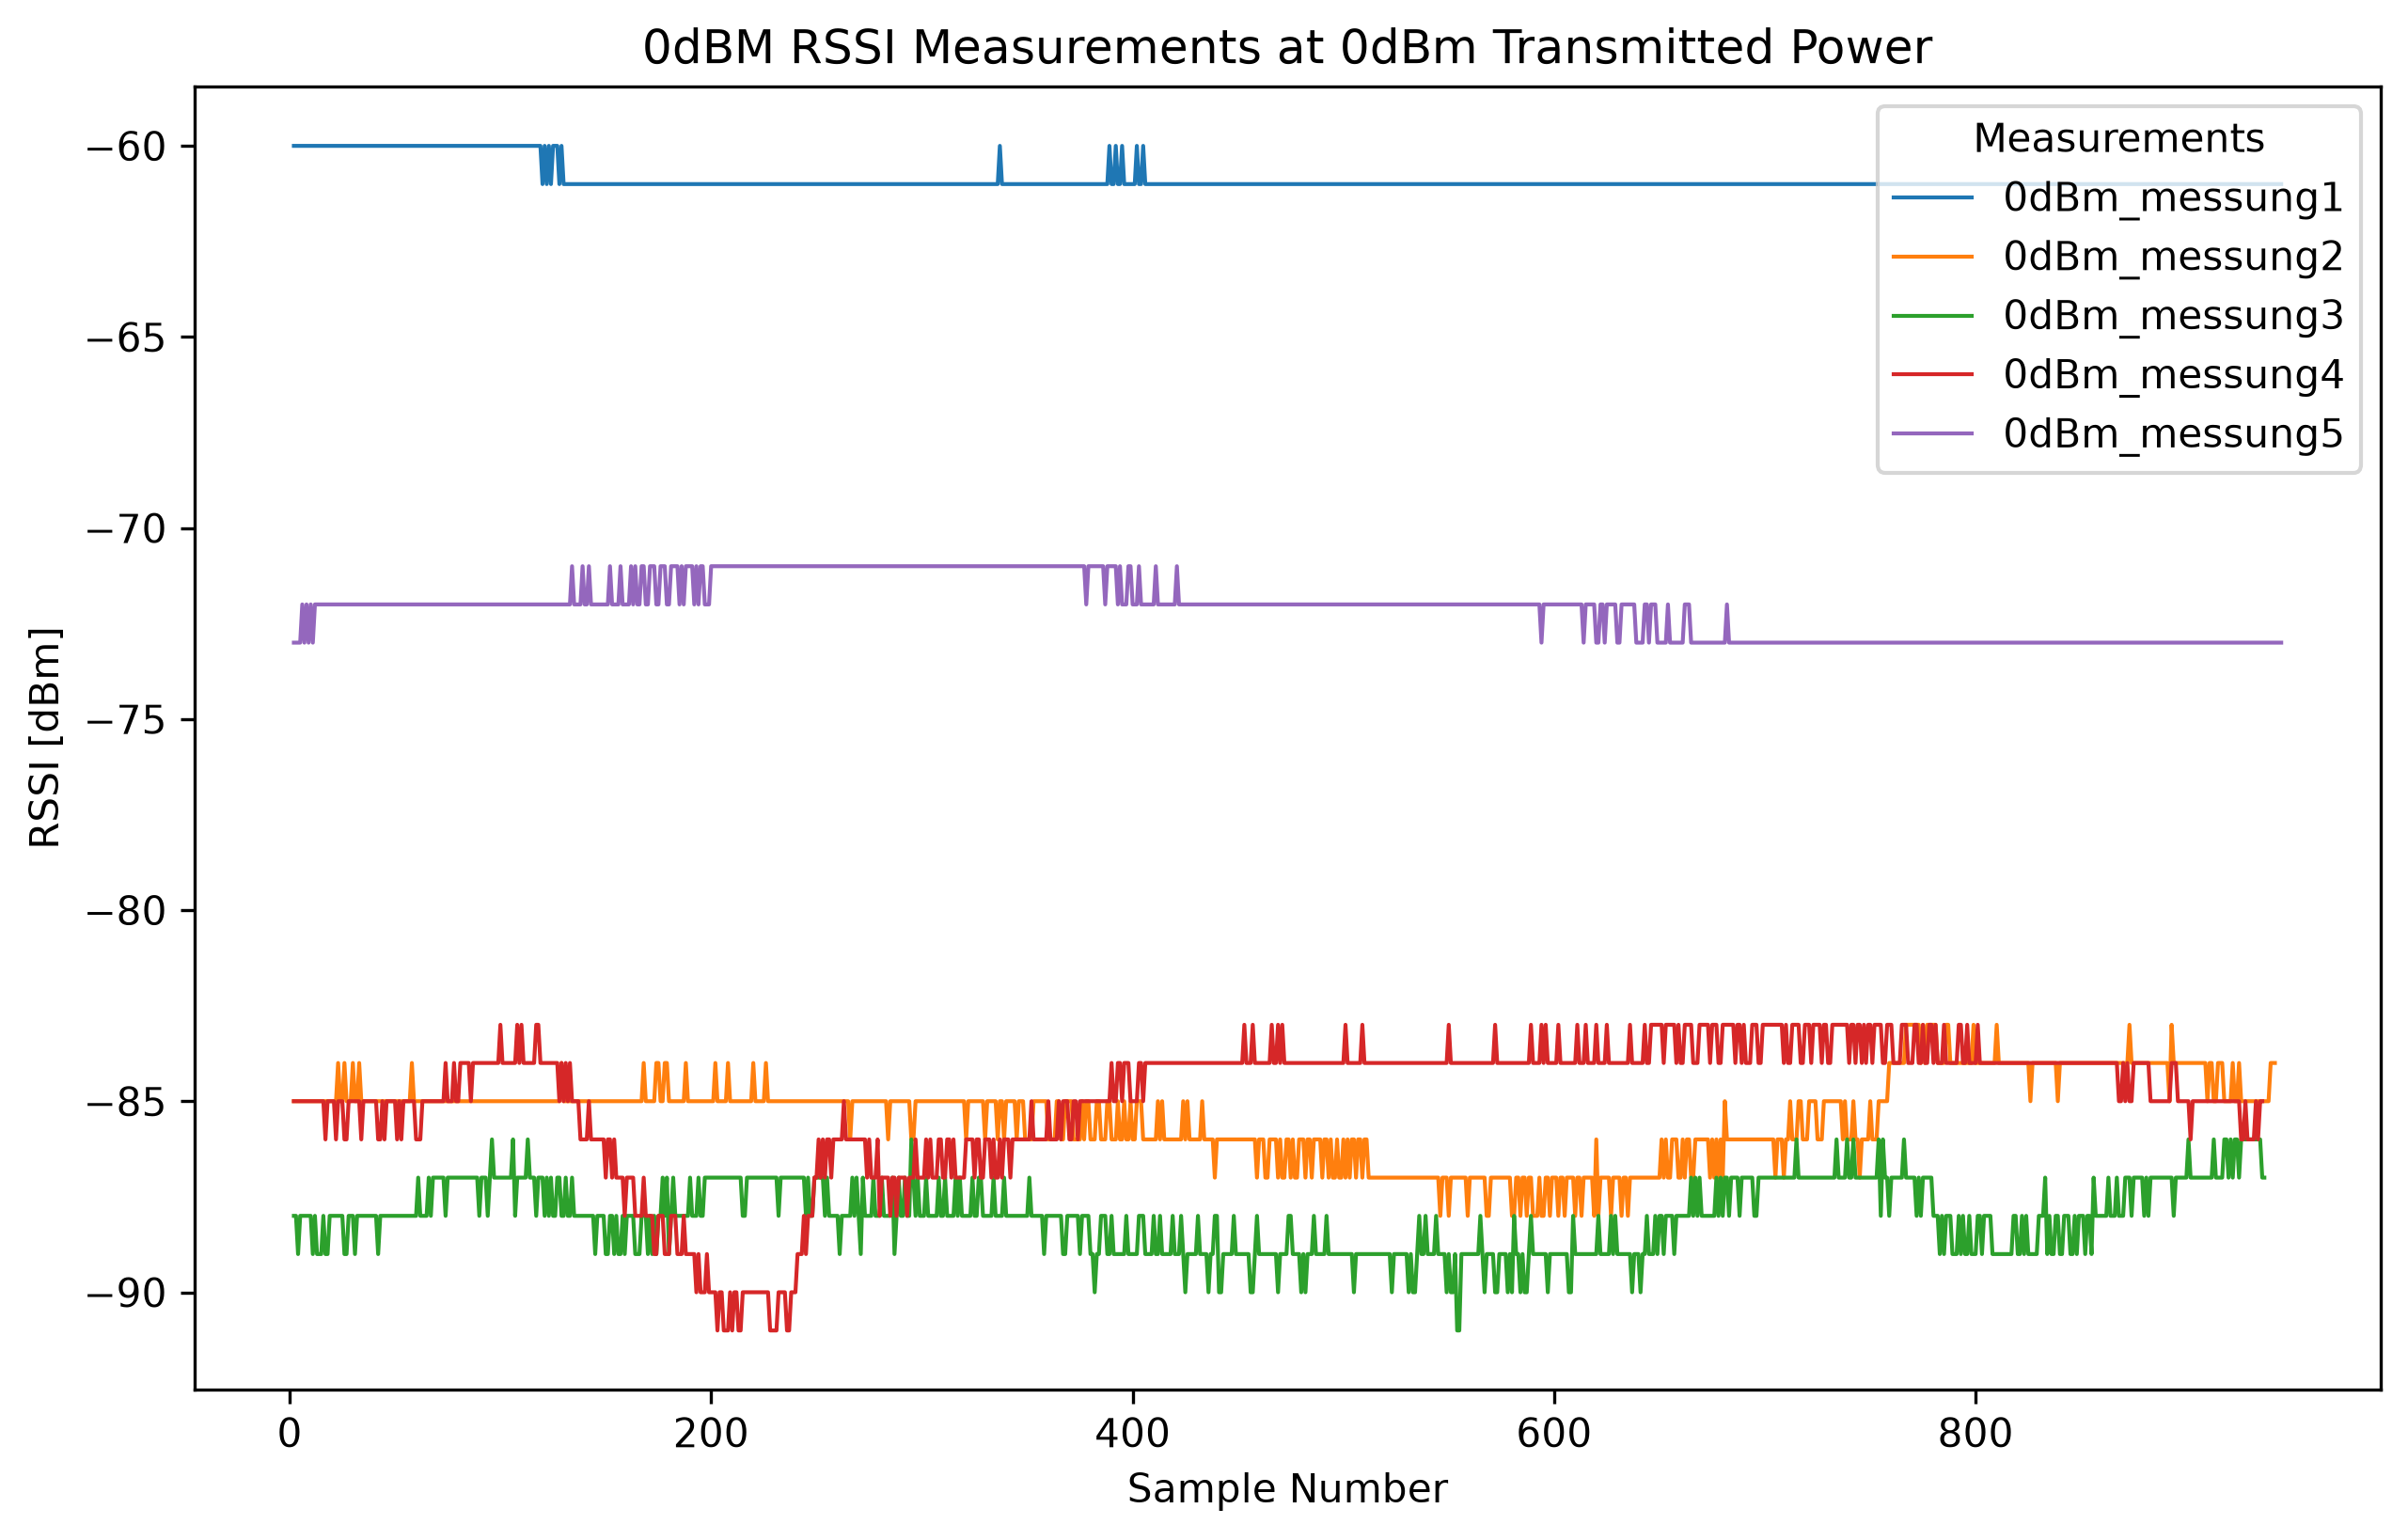
\includegraphics[width=0.92\linewidth]{0dBM_RSSI_Measurements_at_0dBm_Transmitted_Power.png}
    \caption{Received RSSI across 1000 samples for each distance at 0\,dBm transmit power.}
    \label{fig:rssi_samples}
\end{figure}

\begin{itemize}
    \item \textbf{RSSI vs. Distance (Figure~\ref{fig:rssi_samples}):} At 1\,m, the signal remained flat near $-61$\,dBm. Increasing the distance lowered the RSSI to $-72$\,dBm at 4\,m, $-85$\,dBm at 6\,m, $-88$\,dBm at 8\,m, and $-85$\,dBm at 11\,m. Noticeable fluctuations appeared at larger distances due to indoor multipath reflections. The spread of the samples was narrow (1--2\,dBm) at 1\,m and 4\,m and broadened to 5--8\,dBm at 6--11\,m, showing that attenuated signals are much more sensitive to environmental changes.
\end{itemize}

\begin{figure}[htbp]
    \centering
    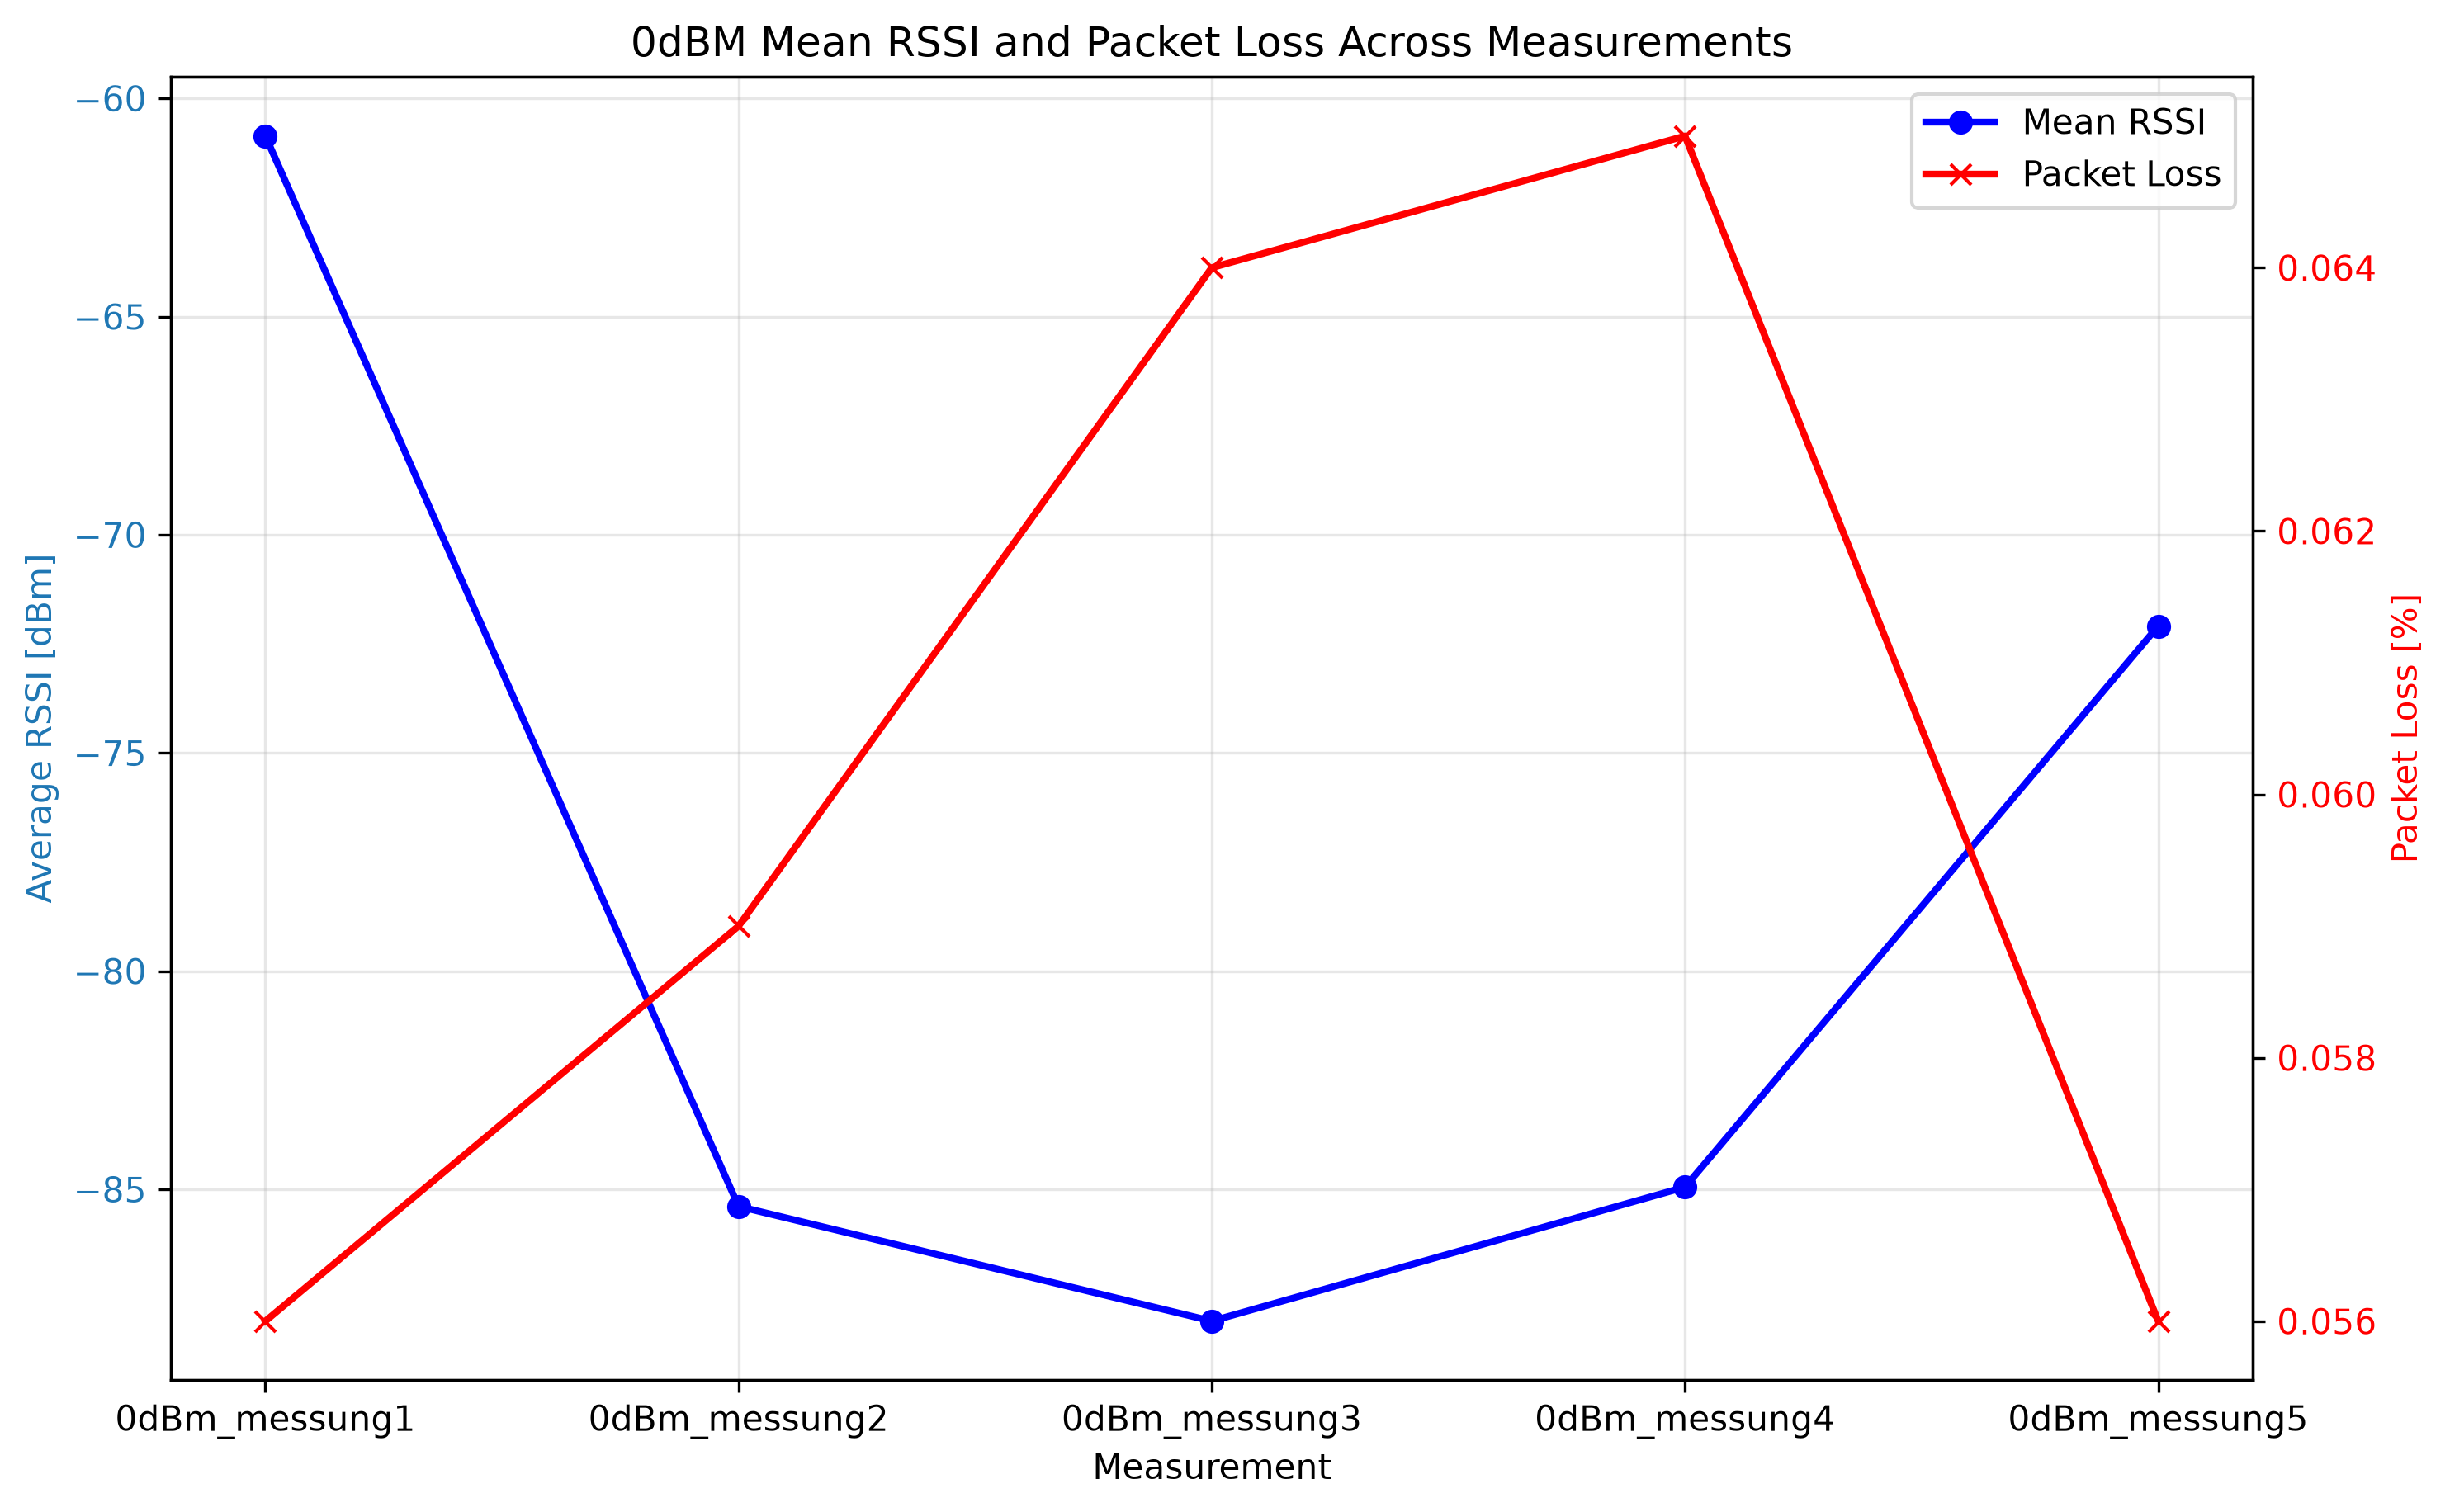
\includegraphics[width=0.85\linewidth]{0dBM_Mean_RSSI_and_Packet_Loss_Across_Measurements.png}
    \caption{Mean RSSI compared with packet loss across all measured distances at 0\,dBm transmit power.}
    \label{fig:mean_rssi_loss}
\end{figure}

\begin{itemize}
    \item \textbf{Packet Reception and Loss (Figure~\ref{fig:mean_rssi_loss}):} Out of 1000 transmitted packets, 945 were received at 1\,m (5.5\% loss) and 942 at 11\,m (5.8\% loss). Despite the $\approx 24$\,dB signal drop from 1\,m to 11\,m, packet loss remained below 6.5\%, showing that 0\,dBm provides ample link margin for indoor spaces.
\end{itemize}

\subsection{Transmit Power at $-40$\,dBm}

\begin{figure}[htbp]
    \centering
    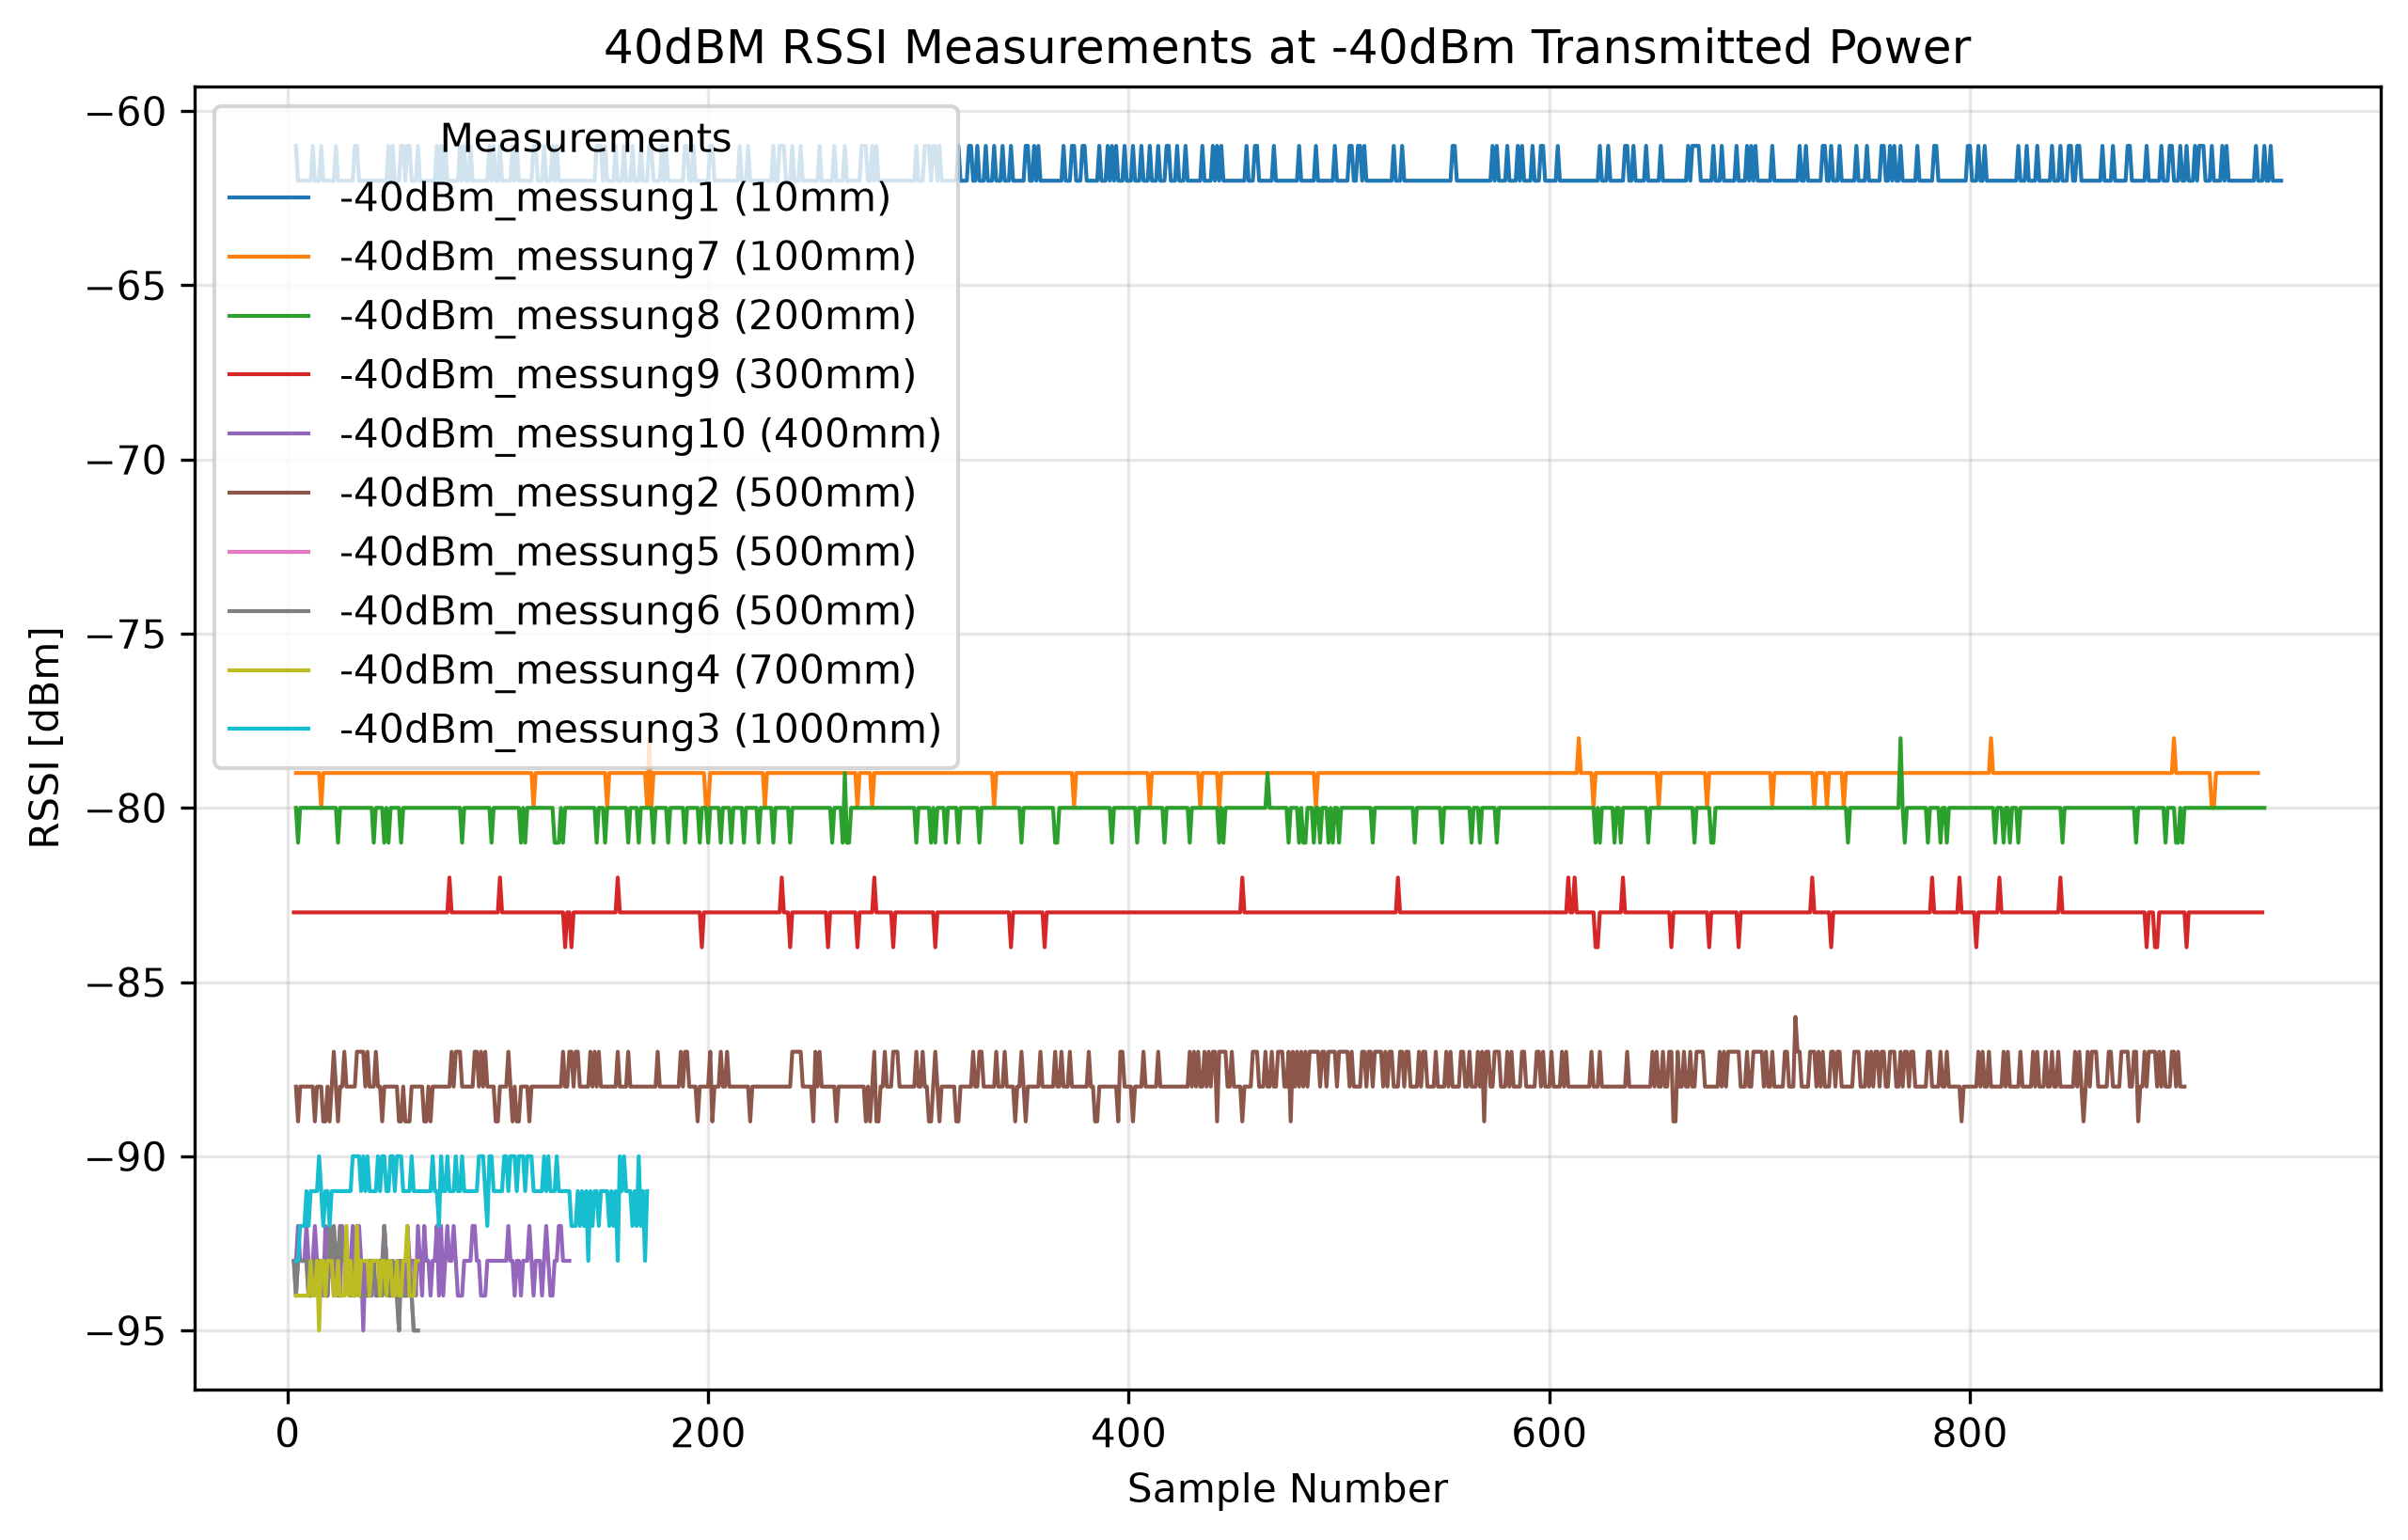
\includegraphics[width=0.92\linewidth]{40dBM_RSSI_Measurements_at_-40dBm_Transmitted_Power.png}
    \caption{Received RSSI across the 1000-packet bursts for each distance at $-40$\,dBm transmit power.}
    \label{fig:rssi_samples_n40}
\end{figure}

\begin{itemize}
    \item \textbf{RSSI Samples (Figure~\ref{fig:rssi_samples_n40}):}
    Up to 300\,mm each run forms a dense, nearly flat trace, while from 400\,mm on the traces break up
    into sparse single points, since only a small fraction of the 1000 packets survives the channel.
\end{itemize}

\begin{figure}[htbp]
    \centering
    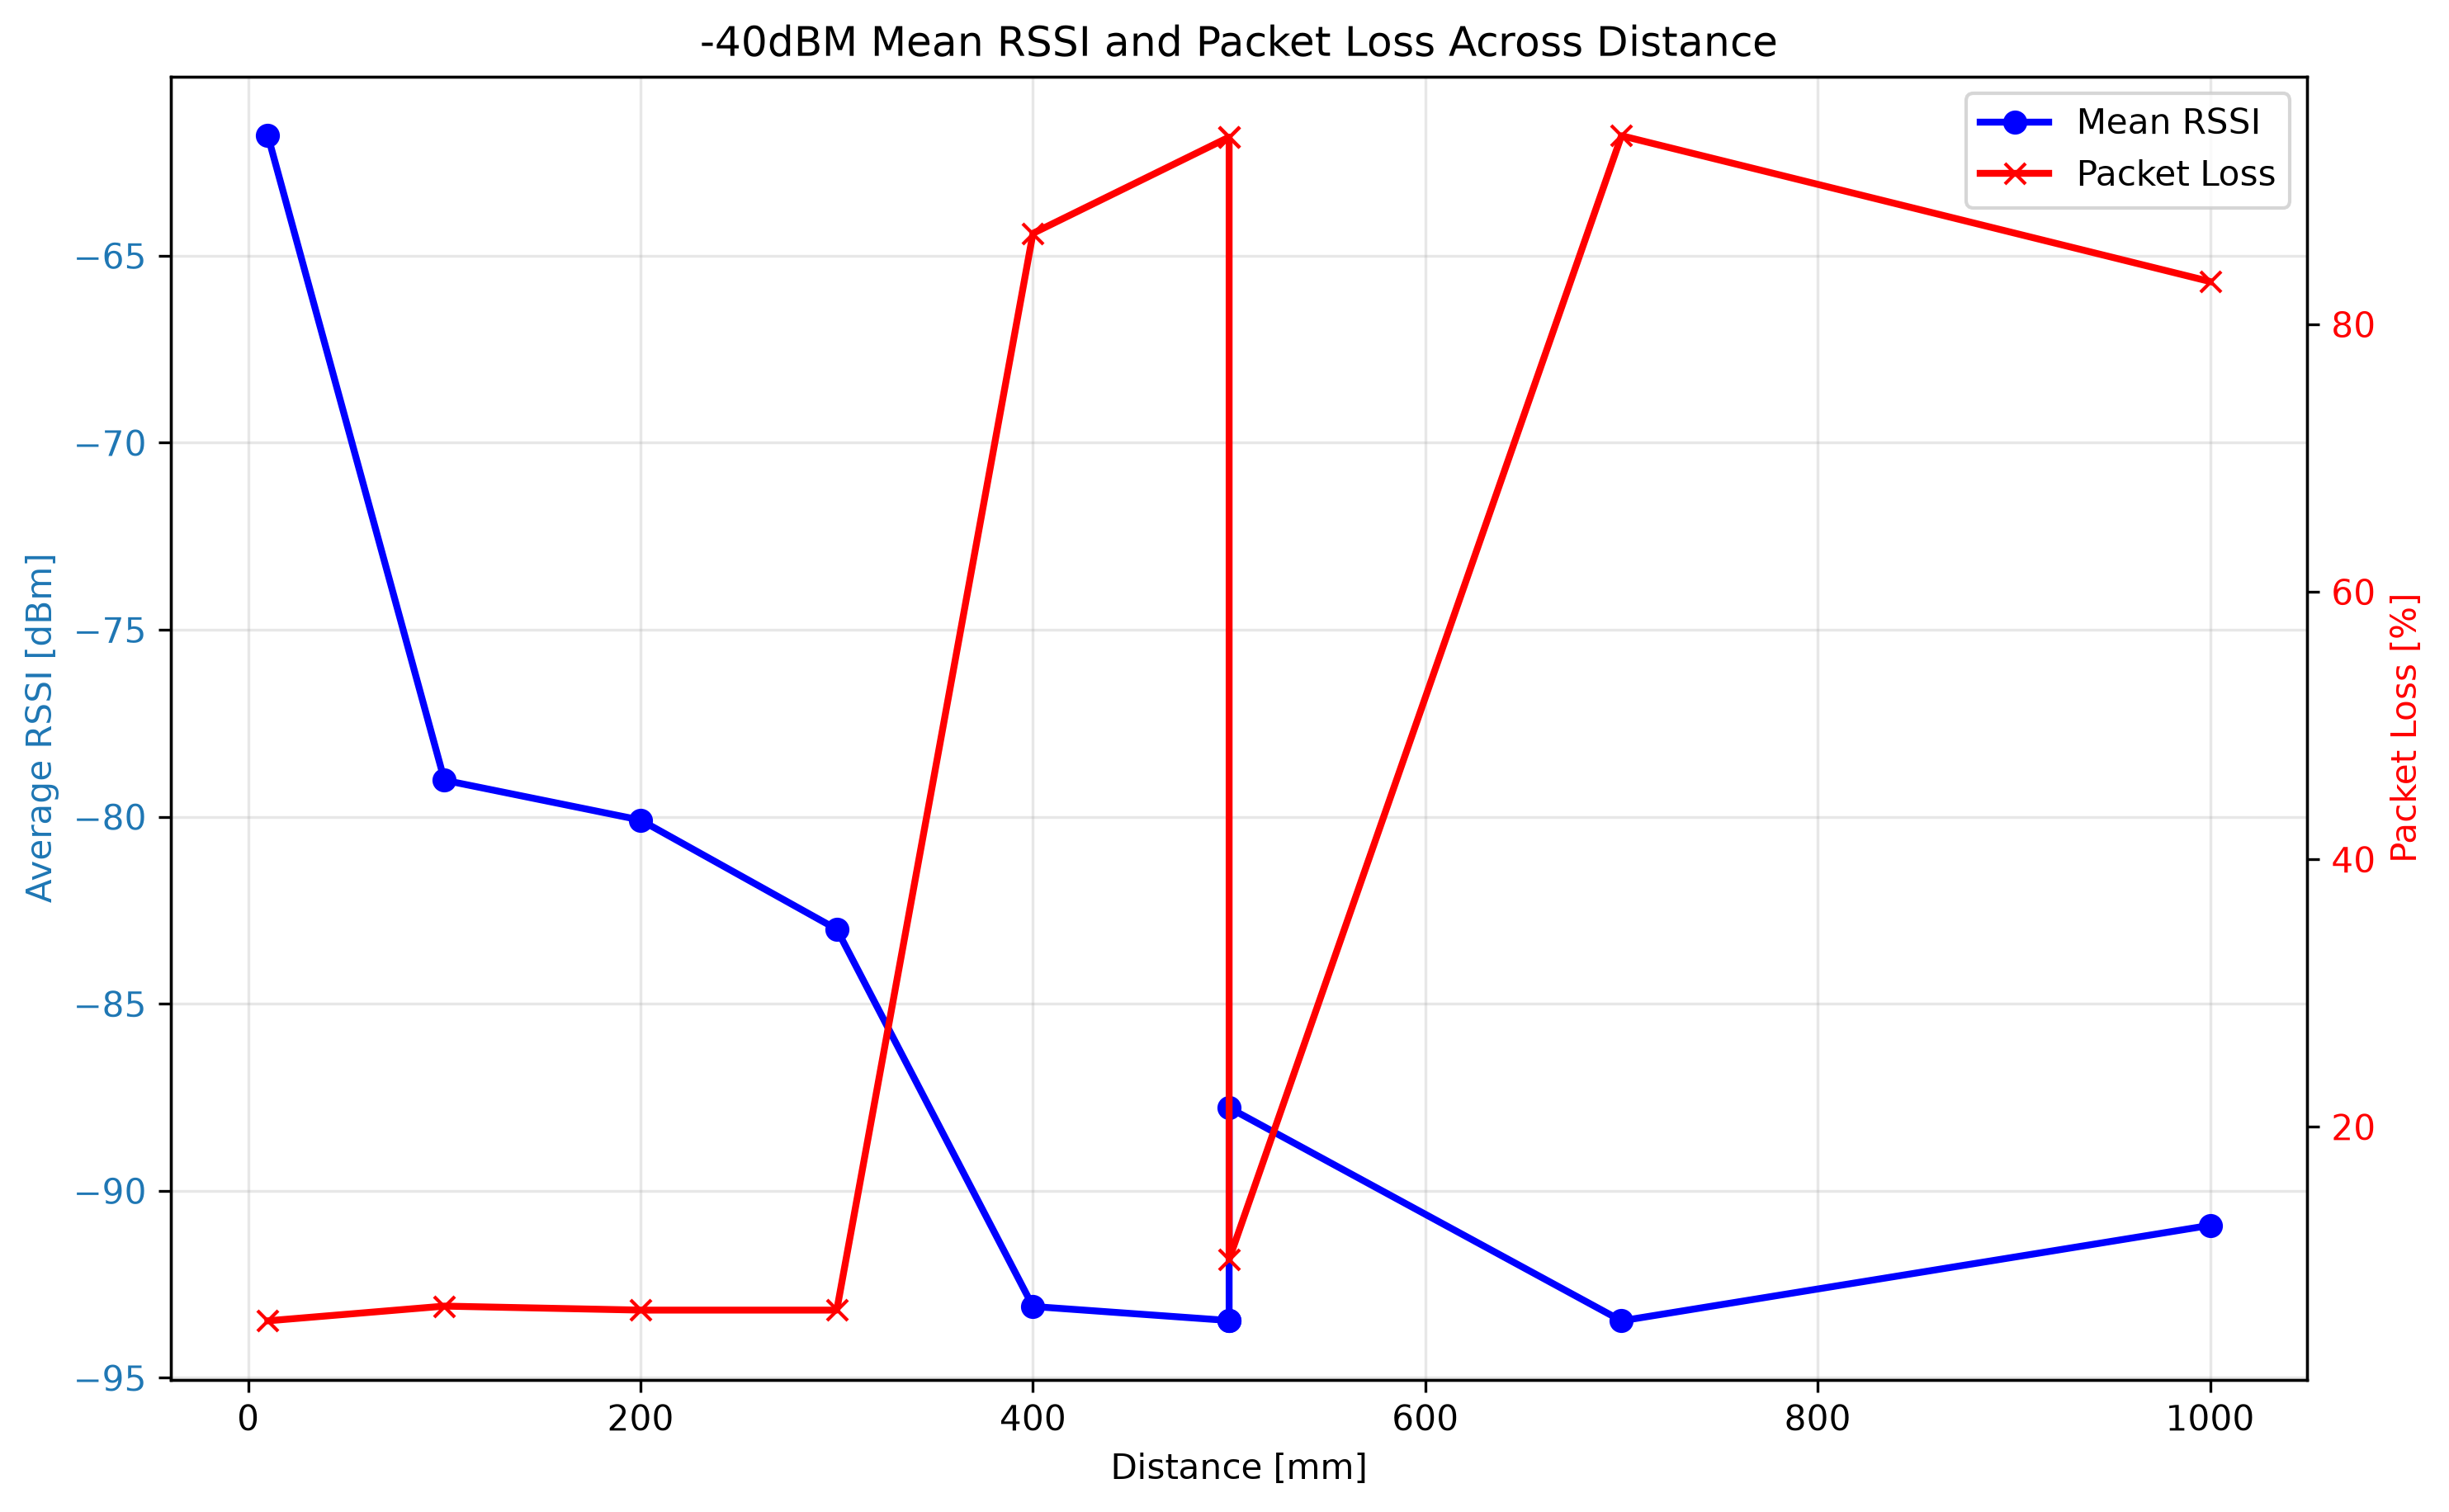
\includegraphics[width=0.85\linewidth]{40dBM_Mean_RSSI_and_Packet_Loss_Across_Distance.png}
    \caption{Mean RSSI compared with packet loss across the measured distances (10\,mm to 1\,m) at $-40$\,dBm transmit power.}
    \label{fig:mean_rssi_loss_n40}
\end{figure}

\begin{itemize}
    \item \textbf{RSSI and Packet Loss (Figure~\ref{fig:mean_rssi_loss_n40}):}
    At 10\,mm the mean RSSI was $-62$\,dBm; between 100\,mm and 300\,mm it stayed above $-83$\,dBm and
    packet loss remained below 7\%. Beyond 300\,mm the link degraded sharply: for most positions at
    400--1000\,mm the mean RSSI fell to $-91$ to $-94$\,dBm and packet loss jumped to 83--94\%.
    The single runs scatter far more than in the 0\,dBm case (e.g., three runs at 500\,mm yielded
    10.1\%, 94.0\%, and 94.0\% loss), because the received power lies close to the receiver sensitivity
    of the 2\,Mbit/s PHY, so small changes in position or phase decide whether a packet is received.
\end{itemize}

\subsection{Comparison of Radio Modes}

The BLE 2\,Mbit/s results at $-40$\,dBm were compared with a second radio mode, IEEE 802.15.4-250\,kbit/s
(\texttt{data\_rate ieee802154\_250Kbit}), at the same transmit power.

\begin{figure}[htbp]
    \centering
    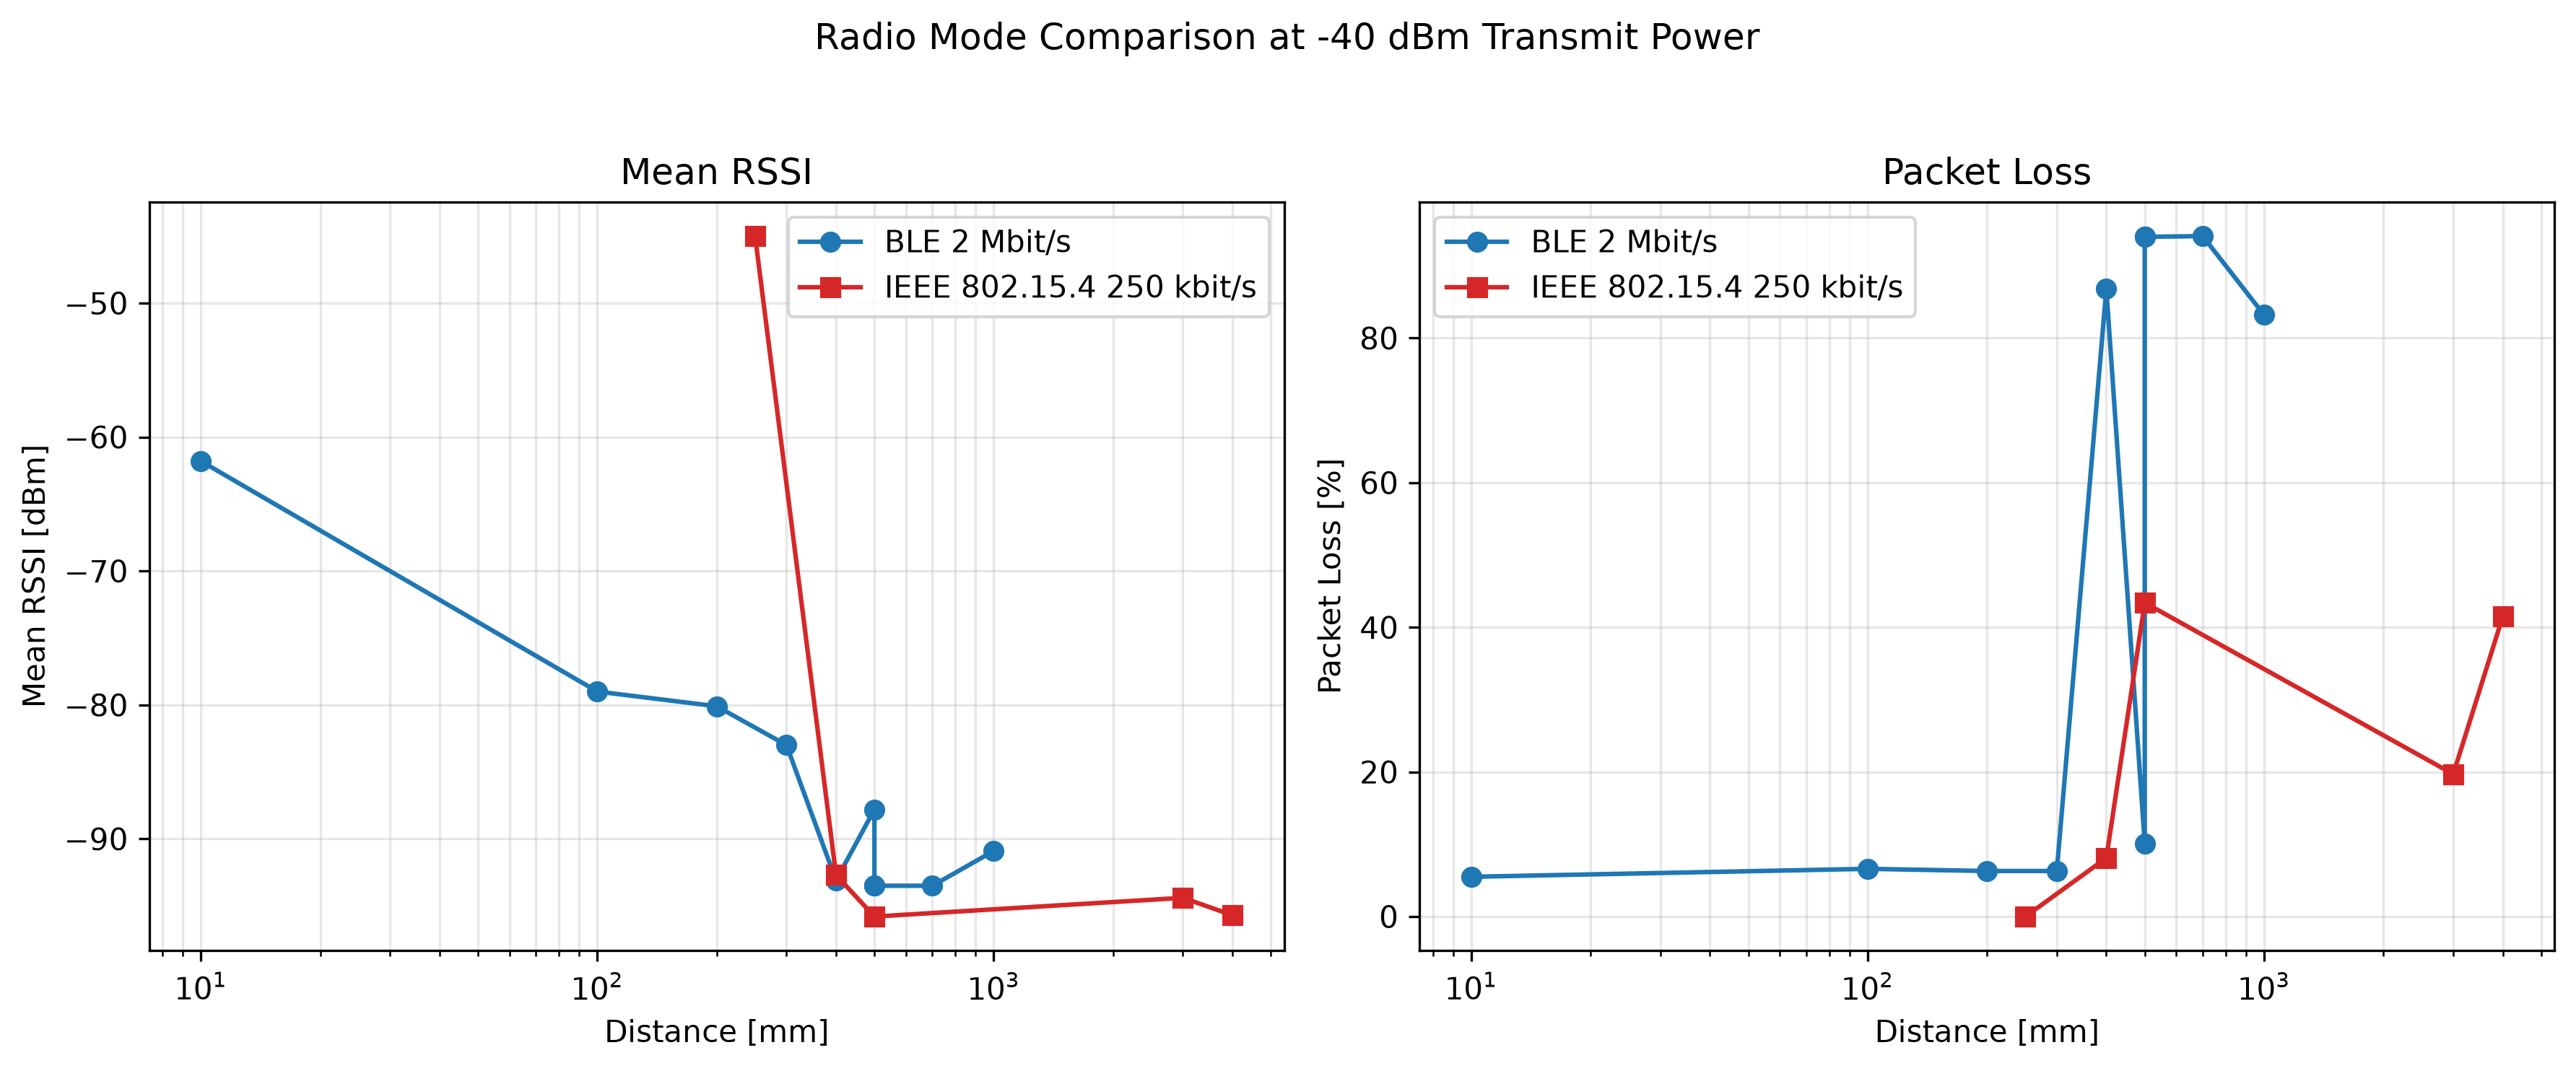
\includegraphics[width=0.95\linewidth]{40dBM_Radio_Mode_Comparison_RSSI_and_Packet_Loss.png}
    \caption{Mean RSSI (left) and packet loss (right) for BLE 2\,Mbit/s and IEEE 802.15.4-250\,kbit/s at $-40$\,dBm transmit power.}
    \label{fig:mode_compare}
\end{figure}

\begin{itemize}
    \item \textbf{Comparison (Figure~\ref{fig:mode_compare}):}
    At 250\,mm the 802.15.4 link was strong and loss-free (1000 of 1000 packets, mean $-45$\,dBm).
    At the common range of 400--500\,mm both modes operated at the sensitivity floor
    ($-92.7$ to $-95.8$\,dBm), but the 250\,kbit/s PHY kept a usable link with 8.1\% and 43.4\% loss,
    while BLE 2\,Mbit/s lost 86.8\% of the packets at 400\,mm: the eight-fold longer symbol time of the
    250\,kbit/s mode provides a clearly better range at the same transmit power. From 400\,mm on, the
    received level of the 802.15.4 session never recovered above $-92$\,dBm, and the session log contains
    the operator note \enquote{winkelmaybebad} (board angle probably misaligned), so the far-range runs
    (3\,m: 19.7\%, 4\,m: 41.5\% loss) are indicative rather than a controlled sweep.
\end{itemize}

\section{Conclusion}

\begin{itemize}
    \item \textbf{Indoor Attenuation:} Physical obstructions and multipath reflections prevent RSSI from decreasing linearly with distance, making raw RSSI unreliable for standalone distance estimation.
    \item \textbf{Link Margin at 0\,dBm:} At 0\,dBm, BLE 2\,Mbit/s easily covers up to 11\,m with negligible loss while the -40\,dBm case had considerably higher packet loss, indicating that higher transmit power is crucial for maintaining reliable links in indoor environments.
    \item \textbf{Data Rate vs.\ Range:} At $-40$\,dBm, the 250\,kbit/s mode kept a usable link at 400\,mm (8.1\% loss) where BLE 2\,Mbit/s was almost entirely lost (86.8\%), confirming that a lower data rate trades throughput for better receiver sensitivity and thus a longer range.
    \item \textbf{Future Implementations:} TODO: conclude what you will consider in future wireless implementations
    (e.g.\ transmit power vs.\ battery life, data rate choice for the required range, and channel selection against interference).
\end{itemize}


%%-----------------------------------------------------------------------------



\printbibliography[heading=noheader]

%%-----------------------------------------------------------------------------
